% Estudo dirigido — Desenvolvimento Colaborativo de Software
% Estilo tipográfico alinhado ao TCC (abnTeX2 + margens/ABNT-UTP).
% Compilar a partir de notas/: pdflatex → bibtex → pdflatex → pdflatex

\documentclass[
    12pt,
    oneside,
    a4paper,
    article,
    section=TITLE,
    sumario=abnt-6027-2012
]{abntex2}

\usepackage{estilo-utp-estudo}
\usepackage{tabularx}
\usepackage{tikz}
\usetikzlibrary{arrows.meta, positioning, calc, shapes.geometric, fit}

\titulo{Estudo dirigido: desenvolvimento colaborativo de software}
\autor{Lucas Muller Scuzziato}
\instituicao{Universidade Tuiuti do Paraná}
\local{Curitiba}
\data{\the\year}
\preambulo{Disciplina Engenharia de Software --- 3 Cs, Git/GitHub, metodologias ágeis e DevOps/CI/CD.}

\begin{document}

\OnehalfSpacing
\setSpacing{1.453}

\imprimircapa

\textual

\section{Conceito de desenvolvimento colaborativo e os 3 Cs}
\label{sec:3cs}

Desenvolvimento colaborativo de software é o processo em que duas ou mais pessoas --- ou times --- trabalham de forma conjunta e interdependente para construir, evoluir e manter um produto de software. Diferentemente do trabalho meramente paralelo (em que cada um entrega uma parte isolada e ``cola'' no fim), a colaboração pressupõe \textbf{interação contínua}: troca de informação, alinhamento de decisões e produção conjunta sobre artefatos compartilhados (código, requisitos, testes, documentação).

Na literatura de \textbf{CSCW} (\textit{Computer-Supported Cooperative Work}) e de engenharia de groupware, essa colaboração é frequentemente analisada pelo \textbf{modelo 3C}, formulado a partir de Ellis, Gibbs e Rein \cite{ellis1991} e sistematizado por Fuks, Raposo, Gerosa e colaboradores \cite{fuks2008}. Nesse modelo, a \textbf{colaboração} é o resultado do \textit{interplay} (interação permanente) entre três dimensões, ilustradas na Figura~\ref{fig:modelo3c}.

\begin{center}
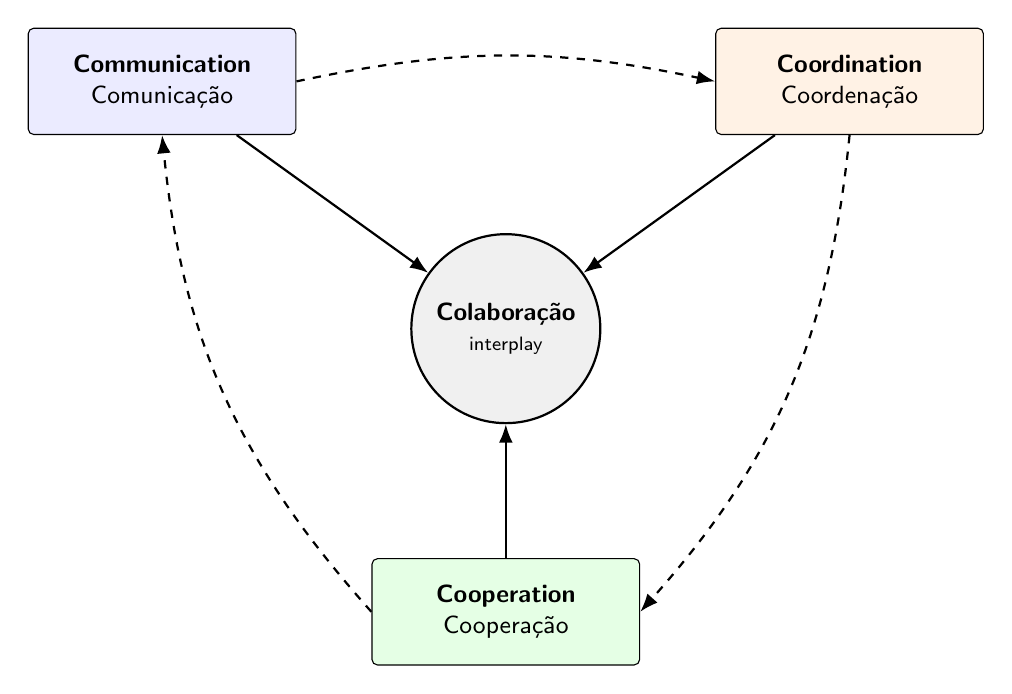
\begin{tikzpicture}[
  font=\small\sffamily,
  box/.style={draw, rounded corners=2pt, align=center, inner sep=6pt, minimum width=3.4cm, minimum height=1.35cm},
  hub/.style={draw, circle, align=center, inner sep=4pt, minimum size=2.4cm, thick},
  arr/.style={-{Latex}, thick}
]
  \node[hub, fill=gray!12] (colab) {\textbf{Colaboração}\\\scriptsize interplay};
  \node[box, fill=blue!8, above left=1.6cm and 1.8cm of colab] (com) {\textbf{Communication}\\Comunicação};
  \node[box, fill=orange!10, above right=1.6cm and 1.8cm of colab] (coo) {\textbf{Coordination}\\Coordenação};
  \node[box, fill=green!10, below=1.7cm of colab] (cop) {\textbf{Cooperation}\\Cooperação};
  \draw[arr] (com) -- (colab);
  \draw[arr] (coo) -- (colab);
  \draw[arr] (cop) -- (colab);
  \draw[arr, dashed] (com.east) to[bend left=12] (coo.west);
  \draw[arr, dashed] (coo.south) to[bend left=18] (cop.east);
  \draw[arr, dashed] (cop.west) to[bend left=18] (com.south);
\end{tikzpicture}
\captionof{figure}{Modelo 3C: colaboração como resultado da interação entre comunicação, coordenação e cooperação.}
\label{fig:modelo3c}
\fonte{Elaboração própria, a partir de Ellis et al. \cite{ellis1991} e Fuks et al. \cite{fuks2008}.}
\end{center}

\subsection{Communication (Comunicação)}

É a troca de mensagens e informações entre pessoas --- negociar significados, esclarecer dúvidas, argumentar decisões e construir entendimento comum. Em software, isso aparece em reuniões, \textit{chats}, comentários em \textit{pull requests}, discussões em \textit{issues}, e-mails e documentação viva. Sem comunicação adequada, o código pode ``compilar'', mas o time deixa de compartilhar a intenção do que está sendo construído.

\subsection{Coordination (Coordenação)}

É a gestão de pessoas, atividades e recursos: quem faz o quê, em que ordem, com quais dependências e prazos. A coordenação organiza o esforço para que a comunicação não se perca e a cooperação aconteça no momento certo. Exemplos típicos: \textit{backlog} priorizado, \textit{sprints}, atribuição de tarefas, políticas de \textit{branch}, papéis (Product Owner, Scrum Master) e regras de \textit{merge}.

\subsection{Cooperation / Collaboration (Cooperação)}

No modelo 3C de Fuks et al. \cite{fuks2008}, \textbf{cooperação} designa a \textit{produção conjunta em um espaço compartilhado} --- operar juntos sobre o mesmo artefato (repositório, \textit{wiki}, quadro Kanban, ambiente de \textit{pair programming}). Já em Ellis et al. \cite{ellis1991}, o termo usado para essa dimensão era \textbf{collaboration}. Por isso a literatura costuma apresentar ``Cooperation / Collaboration'': o nome varia, mas a ideia é a mesma --- trabalho conjunto sobre um \textit{workspace} comum. No modelo brasileiro amplamente citado, \textbf{colaboração} é o fenômeno maior (a combinação dos 3 Cs), e \textbf{cooperação} é a dimensão da produção conjunta \cite{gerosa2004}.

Em resumo: comunicamos para alinhar, coordenamos para organizar, e cooperamos para produzir juntos. Ferramentas e processos de Engenharia de Software sustentam essas três dimensões de forma integrada.

\section{Por que o desenvolvimento de software é colaborativo}
\label{sec:porque}

O software moderno raramente cabe na cabeça --- ou no tempo --- de uma única pessoa. Há pelo menos quatro razões estruturais para isso.

\textbf{Complexidade.} Sistemas reais envolvem requisitos ambíguos, muitas camadas técnicas, integração com serviços externos e evolução contínua. A complexidade obriga a especialização e a revisão cruzada: ninguém domina, sozinho, domínio de negócio, arquitetura, segurança, UX e operação.

\textbf{Divisão de trabalho.} Projetos são decompostos em módulos, \textit{features} e tarefas. Essa divisão só funciona se houver coordenação (dependências, interfaces, definição de ``pronto'') e cooperação sobre o código integrado --- caso contrário, o resultado é um conjunto de peças que não se encaixam.

\textbf{Conhecimento distribuído.} Conhecimento de negócio está com o cliente ou Product Owner; conhecimento técnico está espalhado entre desenvolvedores, QA e operações. O produto emerge da combinação desses saberes, não da soma linear de contribuições isoladas.

\textbf{Qualidade e risco.} Revisões de código, testes em equipe e \textit{feedback} frequente reduzem defeitos e decisões ruins. Colaborar não é só ``ser simpático'': é um mecanismo de engenharia para detectar inconsistências cedo, compartilhar responsabilidade e manter o sistema evolutivo.

Além disso, o contexto atual (times distribuídos, \textit{open source}, produtos digitais com releases contínuos) torna a colaboração mediada por computador a regra, não a exceção --- exatamente o objeto de estudo do CSCW aplicado à Engenharia de Software.

\section{Git, GitHub e o desenvolvimento colaborativo}
\label{sec:git}

Sistemas de controle de versão distribuídos, como o \textbf{Git}, e plataformas como o \textbf{GitHub}, materializam os 3 Cs no fluxo diário do time \cite{chacon2014}. A Figura~\ref{fig:fluxo-git} ilustra um modelo de ramificação (\textit{branching}); a Figura~\ref{fig:mr-plataforma} mostra a tela de um \textit{Merge Request} (análogo ao \textit{Pull Request} do GitHub), com discussão, revisão e integração da mudança.

\begin{center}
\includegraphics[width=0.92\textwidth]{oneflow-git-branching.png}
\captionof{figure}{Modelo de ramificação Git (OneFlow): desenvolvimento em \textit{branches} e integração na linha principal.}
\label{fig:fluxo-git}
\fonte{Wikimedia Commons --- \textit{OneFlow Example.png}, autor Qeef, licença CC BY-SA 4.0. Disponível em: \url{https://commons.wikimedia.org/wiki/File:OneFlow_Example.png}.}
\end{center}

\begin{center}
\includegraphics[width=0.95\textwidth]{gitlab-merge-request.png}
\captionof{figure}{Exemplo de plataforma: \textit{Merge Request} no GitLab (equivalente conceitual ao \textit{Pull Request} do GitHub), com descrição, discussão e revisão.}
\label{fig:mr-plataforma}
\fonte{Wikimedia Commons --- \textit{GitLab Merge Request.png}, GitLab, Inc., licença MIT. Disponível em: \url{https://commons.wikimedia.org/wiki/File:GitLab_Merge_Request.png}.}
\end{center}

\textbf{Histórico e espaço compartilhado (cooperação).} O repositório é o \textit{workspace} comum: cada \textit{commit} registra \textit{quem} mudou \textit{o quê} e \textit{por quê}. O histórico permite auditar decisões, reverter regressões e entender a evolução do produto --- base da cooperação assíncrona.

\textbf{Branches (coordenação + cooperação).} \textit{Branches} permitem trabalhar em paralelo sem destruir a linha principal (\texttt{main}/\texttt{master}). Elas coordenam o isolamento de mudanças (feature, correção, experimento) e, ao mesmo tempo, preparam a cooperação no momento do \textit{merge}.

\textbf{Pull Requests (PRs) e code review (comunicação + cooperação).} O PR é o ponto em que a mudança proposta é discutida: comentários, sugestões e aprovação transformam comunicação em melhoria do artefato compartilhado. O \textit{review} institucionaliza a revisão por pares --- prática colaborativa central de qualidade.

\textbf{Issues e projetos (comunicação + coordenação).} \textit{Issues}, \textit{milestones} e quadros (Projects/Kanban) registram problemas, ideias e tarefas, atribuem responsáveis e acompanham status. São instrumentos de coordenação visível e de memória do time.

Em termos dos 3 Cs: o GitHub não ``substitui'' a colaboração humana; ele \textbf{suporta} comunicação (discussões), coordenação (tarefas, \textit{branches}, políticas de proteção) e cooperação (código e documentação no mesmo repositório). Quem usa só o Git como \textit{backup} pessoal, sem \textit{review}, \textit{issues} ou integração, está subutilizando o potencial colaborativo da ferramenta.

\section{Metodologias ágeis e desenvolvimento colaborativo}
\label{sec:ageis}

O Manifesto Ágil \cite{beck2001} coloca a colaboração no centro: valoriza \textbf{indivíduos e interações} mais que processos e ferramentas, e \textbf{colaboração com o cliente} mais que negociação contratual rígida. As metodologias ágeis não são apenas ``ciclos curtos''; são conjuntos de práticas que forçam os 3 Cs de forma recorrente. A Figura~\ref{fig:scrum} mostra um quadro físico no estilo Scrum/Kanban usado para visualizar o fluxo de trabalho.

\begin{center}
\includegraphics[width=0.92\textwidth]{simple-kanban-board.jpg}
\captionof{figure}{Quadro ágil físico (Scrum/Kanban): colunas de estado e cartões de tarefas visíveis ao time.}
\label{fig:scrum}
\fonte{Wikimedia Commons --- \textit{Simple-kanban-board-.jpg}, autor Jeff.lasovski, licença CC BY-SA 3.0. Disponível em: \url{https://commons.wikimedia.org/wiki/File:Simple-kanban-board-.jpg}.}
\end{center}

\subsection{Scrum}

O Scrum organiza o trabalho em \textit{sprints} com papéis e eventos explícitos. O \textit{Daily Scrum} favorece comunicação rápida sobre progresso e impedimentos; o \textit{Sprint Planning} e o \textit{Backlog} exercem coordenação; a \textit{Sprint Review} e a \textit{Retrospectiva} fecham o ciclo com inspeção conjunta do produto e do processo. O Product Owner conecta o time ao valor de negócio --- colaboração contínua com o ``cliente'' do sistema.

\subsection{Extreme Programming (XP)}

O XP enfatiza práticas de engenharia colaborativa: \textit{pair programming} (dois desenvolvedores no mesmo código --- cooperação intensa), propriedade coletiva do código, integração frequente e \textit{test-driven development}. A ideia é reduzir silos individuais e tornar o conhecimento do sistema patrimônio do time, não de uma única pessoa.

\subsection{Outras práticas ágeis}

Kanban torna o fluxo e os gargalos visíveis (coordenação); \textit{user stories} e critérios de aceite alinham linguagem de negócio e técnica (comunicação); \textit{definition of done} padroniza o que significa ``terminado'' (coordenação + qualidade). Em todos os casos, o ágil trata colaboração como \textbf{disciplina operacional}, não como atributo cultural vago.

\section{DevOps, CI/CD e colaboração entre times}
\label{sec:devops}

Historicamente, desenvolvimento e operações trabalhavam em silos: o time de \textit{dev} ``jogava o build por cima do muro'' e o time de \textit{ops} sofria para colocar em produção. \textbf{DevOps} responde a esse problema cultural e técnico: compartilhar responsabilidade pelo ciclo completo --- do \textit{commit} à operação em produção --- com automação e \textit{feedback} rápido. A Figura~\ref{fig:cicd} apresenta um diagrama de processo de \textit{Continuous Delivery}.

\begin{center}
\includegraphics[width=0.95\textwidth]{continuous-delivery-pipeline.png}
\captionof{figure}{Diagrama de processo de \textit{Continuous Delivery} (pipeline CI/CD): do código à liberação, com etapas automatizadas.}
\label{fig:cicd}
\fonte{Wikimedia Commons --- derivado de \textit{Continuous Delivery process diagram.svg}, autor Grégoire Détrez, licença CC BY-SA 4.0. Disponível em: \url{https://commons.wikimedia.org/wiki/File:Continuous_Delivery_process_diagram.svg}.}
\end{center}

\textbf{Integração Contínua (CI).} Cada mudança integrada ao repositório dispara \textit{build} e testes automatizados. Isso força cooperação diária sobre a linha principal: conflitos e quebras aparecem cedo, quando ainda são baratos de corrigir. A CI é, em essência, colaboração contínua mediada por \textit{pipeline}.

\textbf{Entrega Contínua / Deployment Contínuo (CD).} Estende a CI até deixar o software sempre em estado liberável (ou, no \textit{deployment} contínuo, efetivamente em produção). O \textit{deployment pipeline} \cite{humble2010} dá visibilidade compartilhada do estado de cada mudança --- desenvolvedores, QA e operações passam a operar sobre a mesma evidência.

\textbf{Feedback rápido e integração entre times.} Pipelines, monitoração e alertas fecham o ciclo: defeitos em produção voltam como informação acionável para o time. Isso reforça comunicação entre papéis, coordenação de \textit{releases} e cooperação sobre infraestrutura como código (\textit{Infrastructure as Code}).

Assim, DevOps/CI/CD não são apenas ``ferramentas de automação'': são a extensão da colaboração ágil para além do time de desenvolvimento, incluindo quem mantém o sistema vivo para o usuário final.

\section{Síntese para estudo}
\label{sec:sintese}

\Needspace{12\baselineskip}
\noindent\begin{minipage}{\textwidth}
\centering
\captionof{table}{Exemplos do dia a dia de SE sob a ótica dos 3 Cs.}
\label{tab:sintese}
\begin{tabularx}{\textwidth}{@{}lX@{}}
\toprule
\textbf{Dimensão (3C)} & \textbf{Exemplos no dia a dia de SE} \\
\midrule
Comunicação  & \textit{Issues}, comentários em PR, dailies, revisão com cliente \\
Coordenação  & \textit{Backlog}, \textit{sprints}, \textit{branches}, papéis, Definition of Done \\
Cooperação   & Código no repositório, \textit{pair programming}, \textit{wiki}, pipeline compartilhado \\
\bottomrule
\end{tabularx}
\fonte{Elaboração própria.}
\end{minipage}

Ferramentas (Git/GitHub), métodos (Scrum/XP) e práticas de entrega (DevOps/CI/CD) são camadas complementares do mesmo fenômeno: \textbf{fazer software com e através de outras pessoas}, de forma sustentável e com qualidade.

\postextual
\bibliography{referencias-estudo-colaborativo}

\end{document}
